\documentclass[10pt,twocolumn]{article}
\usepackage[T1]{fontenc}
\usepackage[utf8]{inputenc}
\usepackage{times}
\usepackage[margin=0.75in]{geometry}
\usepackage{amsmath,amssymb}
\usepackage{graphicx}
\usepackage{booktabs}
\usepackage{array}
\usepackage[numbers,sort&compress]{natbib}
\usepackage[hidelinks]{hyperref}
\usepackage{xcolor}
\graphicspath{{figures/}}
\setlength{\columnsep}{0.25in}
\setlength{\tabcolsep}{3.5pt}
\newcommand{\gam}{\gamma}
\newcommand{\Lz}{L0}

\title{The SAE Decoder Power-Law Exponent Is Not a Property of a Layer:\\
a Re-measurement on 288 Gemma Scope Autoencoders}
\author{Anonymous authors}
\date{}

\begin{document}
\maketitle

\begin{abstract}
\citet{li2025geometry} found that the covariance of sparse autoencoder (SAE) decoder directions has a power-law eigenspectrum, and that its exponent is steepest in the middle layers of Gemma-2-2B. We reproduce their three slopes to within 0.02\% and re-measure the exponent on 288 Gemma Scope SAEs that span 26 layers, 7 widths (16k to 1M latents) and L0 from 9 to 457 active latents per token. In the rank window they fitted, L0 accounts for most of the variation: in a regression on log L0, layer and log width, removing L0 lowers $R^2$ by 0.65, removing layer by 0.26 and removing width by 0.001. At layer 12 the slope flattens by 0.099 per doubling of L0 across seven widths ($R^2$ = 0.98), and changing only $k$ in our own TopK SAEs at layer 13 gives 0.092 per doubling. At matched L0 the mid-stack peak remains in the top 150 eigendirections, but the contrast between layers 12 and 24 that Li et al.\ report shrinks from 0.21 to 0.16, and in ranks 31--1000 the steepest layers are 2--7. Dividing by the activation covariance's slope rescales the L0 dependence without removing it. Activation spectra are steeper than decoder spectra at all 26 layers under raw and per-token-normalised preprocessing; only standardising each residual dimension brings them level, which is the one reading under which Li et al.'s remark that activations decay more slowly can hold. We also measure the estimator's own biases: a bias set by the number of live latents, covariance slopes that come out 0.10--0.14 too steep in the bulk when estimated from 200k tokens, and 5--8 effective samples behind 26-layer correlations. Removing near-duplicate latents or latents aligned with massive activations moves the slope by at most 0.012 in the top windows. We close with a reporting checklist for this statistic.
\end{abstract}

\section{Introduction}
\label{sec:intro}

The eigenspectrum of an SAE's decoder directions is a cheap, model-wide summary of how a dictionary is arranged. \citet{li2025geometry} computed it for Gemma Scope SAEs \citep{lieberum2024gemmascope}, found that the sorted eigenvalues of the decoder-row covariance follow a power law, and reported that its slope depends on depth: $-0.47$ at layer 12 against $-0.24$ at layer 0 and $-0.25$ at layer 24 for the three SAEs in their released notebook. Read this way, the exponent measures something about the layer. We argue that it mostly does not. In the window Li et al.\ fitted, the exponent of a Gemma Scope decoder is set first by the SAE's sparsity (L0, the mean number of active latents per token), second by layer, and barely by width; the layer pattern itself changes shape with the rank window, because the spectrum is curved; and the three SAEs Li et al.\ compared differ in L0. A layer contrast read off this statistic is therefore partly a sparsity contrast, and any number quoted without its L0 and rank window cannot be compared with another.

The question matters because the statistic is easy to compute and is starting to be reused. \citet{peter2025progressive} replicated the power law on TopK SAEs and found that their larger SAEs decay less steeply, but their larger SAEs also had larger $k$, so width and sparsity were confounded. We separate the two, and the other choices an analyst makes, on a population large enough to do so.

\paragraph{Contributions.}
\begin{enumerate}
\setlength{\itemsep}{1pt}
\item An exact reproduction of Li et al.'s slopes, and a decomposition of the exponent over 288 Gemma Scope SAEs into L0, layer and width effects in four rank windows (Section~\ref{sec:what}), with a controlled sweep of $k$ in our own TopK SAEs at a fixed layer.
\item Li et al.'s layer comparison redone at matched L0: about a quarter of the layer-12 to layer-24 contrast in their window is an L0 difference, and the mid-stack peak is specific to the top of the spectrum.
\item The exponent relative to the activation covariance $\Sigma$ (Section~\ref{sec:gamma}): at one layer this ratio obeys the same L0 law rescaled by a constant, and $\Sigma$ is steeper than the decoder spectrum at every layer unless each dimension is standardised, which reconciles our measurements with Li et al.'s remark about activation spectra.
\item The estimator's properties (Section~\ref{sec:estimator}): its dependence on the number of live latents, on how many tokens $\Sigma$ is estimated from, on window overlap, and the small effective sample size of correlations across layers. We list what the exponent does not reflect (Section~\ref{sec:not}) and give a reporting checklist (Section~\ref{sec:discussion}).
\end{enumerate}

\section{Related work}
\label{sec:related}

\citet{li2025geometry} describe SAE feature structure at three scales; the power-law decoder spectrum is their largest (``galaxy'') scale. They fit the leading eigenvalues after reducing to 100 principal components; their released notebook fits ranks 11--150 of the full spectrum, which is the window we reproduce. They also compare activation spectra with SAE-feature spectra and report that activations decay more slowly. \citet{peter2025progressive} replicate the decoder power law on TopK SAEs (exponents $-0.54$ to $-0.72$), with the width--$k$ confound noted above. \citet{michaud2025manifolds} model how an SAE allocates latents to features of different frequencies; their exponent describes latents per feature, not a decoder eigenspectrum, so any link to the spectrum is an extension we do not test here.

The SAEs we analyse are Gemma Scope JumpReLU SAEs \citep{rajamanoharan2024jumprelu, lieberum2024gemmascope}; our own SAEs use the TopK recipe with the AuxK loss \citep{gao2024scaling}. Power-law covariance spectra and anisotropy of the representations themselves are well documented \citep{ghosh2022powerlaws, ethayarajh2019contextual}, which is why we also express the decoder exponent relative to $\Sigma$. \citet{saraswatula2025whitening} argue that SAEs trained on unwhitened inputs are biased toward high-variance directions and show that whitening helps; we do not train on whitened inputs in this version (Section~\ref{sec:gamma}). Comparing an SAE statistic with matched nulls has precedents: random-model baselines \citep{heap2025random}, frozen-random SAE components \citep{korznikov2026sanity}, and i.i.d.\ code controls for a different decoder statistic \citep{borobia2026nearfloor}. Our candidate confounds come from known SAE and transformer phenomena: feature splitting and absorption \citep{chanin2025absorption}, dense latents \citep{sun2025dense} and massive activations \citep{sun2024massive}. \citet{prieto2026correlations} show in toy models that data correlations shape learned feature geometry, a mechanism consistent with the covariance dependence we report but not tested here.

\section{Setup}
\label{sec:setup}

\paragraph{SAEs and L0.} We use the decoder matrices of 288 Gemma Scope residual-stream SAEs for Gemma-2-2B: all 135 at width 16k and all 135 at width 65k (5--6 L0 values at each of 26 layers), plus 18 more at layer 12 with widths 32k, 131k, 262k, 524k and 1M. L0 is the mean number of active latents per token. For Gemma Scope we use the L0 in each SAE's release name, the only value available for all 288. We measured L0 for all 135 16k SAEs on 32,736 Pile tokens: measured over named L0 lies between 0.85 and 1.12. At layer 12 we use L0 measured on 1M tokens for the 22 SAEs where we have it. For TopK SAEs, L0 equals $k$.

\paragraph{The exponent.} For a decoder matrix with unit-norm rows (Gemma Scope rows have norm $1 \pm 3\times10^{-7}$), we take the centred covariance of the rows, sort its eigenvalues $\lambda_1 \ge \lambda_2 \ge \dots$, and fit $\log_{10}\lambda_i$ against $\log_{10} i$ by least squares over a rank window. We call the fitted coefficient the \emph{slope} (negative; more negative is steeper). It never depends on any estimate of the activation covariance. Rows of dead latents are included, as in Li et al.'s notebook.

\paragraph{Rank windows.} Because the log--log spectrum is curved, the slope depends on the window. We report four windows fixed before the analysis: ranks 4--50 and 11--150 (the \emph{top} windows; 11--150 is the primary window and the one in Li et al.'s notebook), and ranks 31--450 and 101--1000 (the \emph{bulk} windows). The windows overlap: ranks 11--150 contain 40 of the 47 ranks of 4--50, and 120 of the 420 ranks of 31--450. Agreement across adjacent windows is therefore not independent confirmation.

\paragraph{Activation covariance and $\gam$.} $\Sigma$ is the covariance of residual-stream activations (after the block, beginning-of-sequence token dropped), estimated from 1M tokens of the Pile at context 1,024 for each of the 26 layers. We define $\gam$ as the decoder slope divided by $\Sigma$'s slope in the same window, so $\gam = 1$ means the decoder spectrum falls as steeply as the activation spectrum. Our own SAEs use the $\Sigma$ of their 10M training tokens.

\paragraph{Our TopK SAEs.} At layer 13 we trained 16k-wide TopK SAEs at $k$ = 1, 2, 4, 8, 16, 40 and 128 (2 seeds each) on 9.5M cached tokens for 3 epochs. At layers 3, 13 and 23 we trained 16k and 65k SAEs at $k = 40$ (3 seeds) on real activations and on a Gaussian $N(\mu,\Sigma)$ with the same mean and covariance. Appendix~\ref{app:methods} gives the hyperparameters.

\paragraph{Reproduction.} Applying this computation to the three SAEs in Li et al.'s notebook (65k; L0 73, 72 and 124 at layers 0, 12 and 24) gives $-0.2383$, $-0.4684$ and $-0.2545$, equal to their values to within 0.02\% (Table~\ref{tab:repro}). Centring changes the slope by at most 0.0007, and normalising rows changes nothing.

\section{What sets the exponent}
\label{sec:what}

\begin{figure*}[t]
\centering
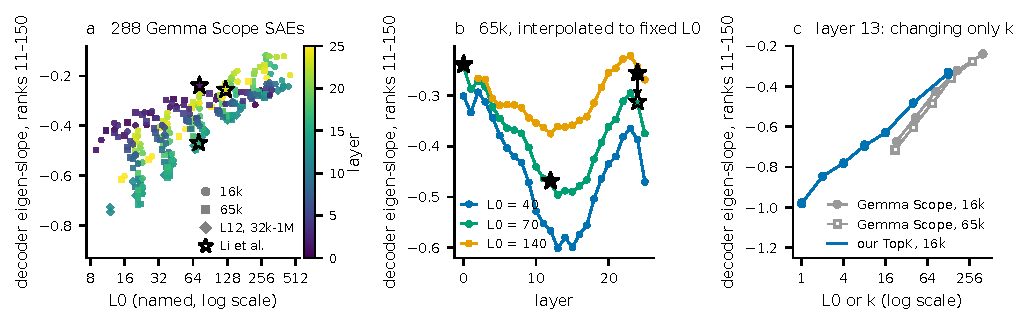
\includegraphics[width=\textwidth]{thesisB_fig1_sparsity_layer.pdf}
\caption{\textbf{L0 moves the exponent more than layer does.} Ranks 11--150. (a) Slope against L0 for all 288 Gemma Scope SAEs, coloured by layer; the three SAEs Li et al.\ compared are starred. Within a layer, the slope flattens steadily with L0; across layers at one L0, points spread by less. (b) Slope against layer for 65k SAEs interpolated to L0 = 40, 70 and 140 (140 is missing at two layers). Filled stars: Li et al.'s SAEs at their own L0 (73, 72, 124). The open star is layer 24 interpolated to L0 = 72: matching L0 moves it from $-0.254$ to $-0.312$. (c) Layer 13: our TopK SAEs at $k$ = 1--128 (2 seeds; open circles have under 2,000 live latents) and Gemma Scope's 16k and 65k ladders. Changing only $k$ reproduces the L0 dependence at a similar rate.}
\label{fig:main}
\end{figure*}

\subsection{L0 dominates in the top windows}

We regress the slope of each of the 288 SAEs on $\log_2$ L0, layer (26 categories) and $\log_2$ width, and ask how much $R^2$ each term carries when the others are present (Table~\ref{tab:decomp}). In the two top windows, removing L0 lowers $R^2$ by 0.73 and 0.65, removing layer by 0.21 and 0.26, and removing width by at most 0.003. The additive model explains 0.89--0.91 of the variance; letting the L0 effect differ by layer raises this to 0.97--0.98. Holding layer and width fixed, each doubling of L0 flattens the slope by 0.081 in ranks 11--150. Over the L0 range Gemma Scope spans (5.7 doublings), this is 0.46, against a 0.21 spread of layer effects at fixed L0 and 0.025 for width over six doublings. Figure~\ref{fig:main}a shows the same thing directly: at a fixed L0, layers spread by less than one layer's own L0 ladder does.

\begin{table}[t]
\centering
\small
\caption{\textbf{Variance in the slope over 288 SAEs, by term.} OLS of slope on $\log_2$ L0, layer (categorical) and $\log_2$ width. ``Alone'': $R^2$ of a model with that term only. ``Drop'': loss in $R^2$ when the term is removed from the additive model. $b$: change in slope per doubling of L0. Layer range: spread of the fitted layer effects at fixed L0.}
\label{tab:decomp}
\begin{tabular}{lcccc}
\toprule
 & 4--50 & 11--150 & 31--450 & 101--1000 \\
\midrule
$R^2$, L0 alone & 0.69 & 0.62 & 0.49 & 0.29 \\
$R^2$, layer alone & 0.16 & 0.22 & 0.49 & 0.64 \\
Drop L0 & 0.73 & 0.65 & 0.46 & 0.28 \\
Drop layer & 0.21 & 0.26 & 0.47 & 0.62 \\
Drop width & 0.003 & 0.001 & 0.001 & 0.010 \\
$R^2$, additive & 0.91 & 0.89 & 0.95 & 0.92 \\
$R^2$, + L0$\times$layer & 0.97 & 0.98 & 0.97 & 0.96 \\
$b$ per doubling & 0.090 & 0.081 & 0.062 & 0.056 \\
Layer range & 0.21 & 0.21 & 0.25 & 0.34 \\
\bottomrule
\end{tabular}
\end{table}

Two checks bear on this decomposition. Named and measured L0 differ by up to 15\%, so we refit the 135 16k SAEs with measured L0: the per-doubling coefficient moves from 0.077 to 0.080 in ranks 11--150 and the $R^2$ of the L0-plus-layer model by at most 0.011 (Appendix~\ref{app:methods}). Second, the L0 effect is not uniform across layers. Within single 16k ladders it ranges from 0.021 per doubling at layer 2 to 0.129 at layer 15 (median 0.083). The mid-stack layers are the most sensitive to sparsity, so the layer contrast depends on which L0 it is read at.

\subsection{At one layer: a log-linear law in L0, flat in width}

At layer 12 Gemma Scope released 28 SAEs over seven widths. Their slope in ranks 11--150 rises from $-0.745$ at L0 = 13 to $-0.242$ at L0 = 444, fitted by
\begin{equation}
\text{slope} = -1.086 + 0.099\,\log_2 \text{L0} \quad (R^2 = 0.98).
\label{eq:l12}
\end{equation}
Li et al.'s $-0.468$ is one point on this line. The same form holds in ranks 4--50 (0.099 per doubling, $R^2$ 0.97) and 31--450 (0.058, $R^2$ 0.95) and fails in ranks 101--1000 (0.038, $R^2$ 0.65), where the seven widths separate (Figure~\ref{fig:windows}, bottom). At matched L0, width moves the slope by at most 0.051 in ranks 11--150 over six doublings at L0 = 40 and 70 (0.063 at L0 = 20, three widths), and by 0.062--0.089 in ranks 4--50. In ranks 101--1000 it moves it by 0.115--0.144. Part of that deep-window width effect is the estimator: cutting a 1M-wide decoder to 16,384 random rows moves its ranks 101--1000 slope 28--51\% of the way to the 16k SAE at similar L0 (Section~\ref{sec:estimator}).

\subsection{Changing only the sparsity}

The Gemma Scope ladders differ in more than L0: each was trained with its own sparsity coefficient. Our TopK sweep at layer 13 changes only $k$, with the same data, width, optimiser and seeds. The slope in ranks 11--150 runs from $-0.979$ at $k = 1$ to $-0.335$ at $k = 128$, flattening by 0.089 per doubling over $k$ = 1--128 ($R^2$ = 0.994) and by 0.092 over $k$ = 8--128 (Figure~\ref{fig:main}c; seed spread at most 0.014). Gemma Scope's layer-13 ladders flatten by 0.106 (16k) and 0.121 (65k) per doubling. The recipes differ in level: at $k = 40$ our slope is $-0.482$, against $-0.568$ for Gemma Scope 16k at L0 = 40. So the rate is similar across recipes and the intercept is not. At $k \le 2$ fewer than 2,000 of 16,384 latents are alive, which biases the slope (Section~\ref{sec:estimator}).

\subsection{Layer at matched L0, and Li et al.'s comparison}

With L0 held fixed by interpolation along each layer's ladder, the top-window slope still peaks mid-stack (Figure~\ref{fig:main}b). For 16k SAEs in ranks 11--150 the steepest layer is 13 at L0 = 40 and 70, and the spread across layers is 0.242 at L0 = 40, 0.186 at L0 = 70 and 0.161 at L0 = 140. For 65k SAEs it is 0.309 and 0.254 at L0 = 40 and 70. The peak is real but its size depends on the L0 at which it is read.

Li et al.'s layer-0 and layer-12 SAEs have matched L0 (73 and 72), and their contrast of 0.230 stands. Their layer-24 SAE has L0 = 124. Interpolating layer 24's 65k ladder to L0 = 72 gives $-0.312$ instead of $-0.254$, so the layer-12 to layer-24 contrast falls from 0.214 to 0.156 in ranks 11--150. About a quarter (0.058) of it is an L0 difference. The same holds in the other windows (shrinkage 0.04--0.05, 17--27\%).

\subsection{The window decides what the layer profile looks like}

\begin{figure*}[t]
\centering
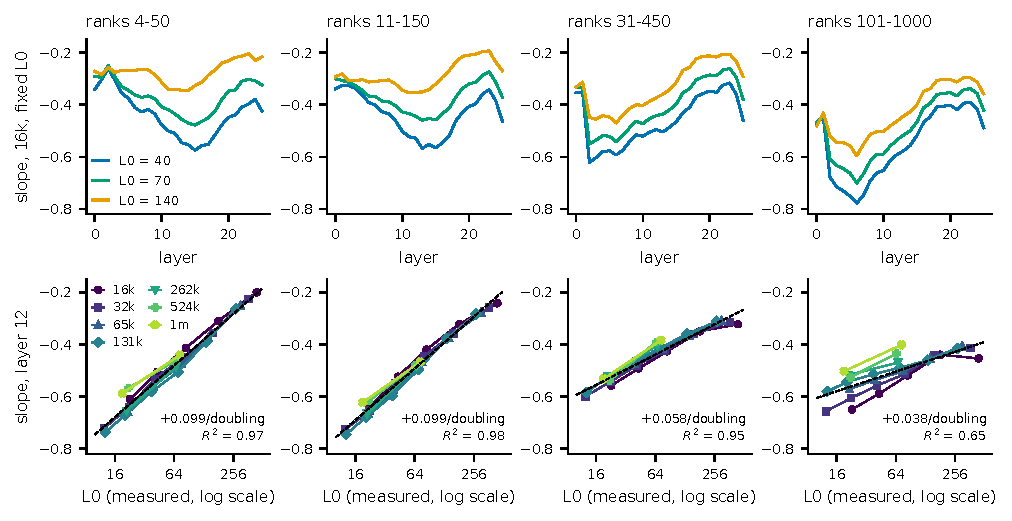
\includegraphics[width=\textwidth]{thesisB_fig2_windows.pdf}
\caption{\textbf{The rank window changes the layer pattern; width matters little except deep in the spectrum.} Top: slope against layer for 16k SAEs at L0 = 40, 70 and 140, one panel per window. In the top windows the slope peaks at layers 13--15; in the bulk windows it is steepest at layers 2--7 and flattens with depth. Bottom: layer 12, slope against measured L0 for 28 SAEs at seven widths, with the pooled log-linear fit (dashed). The widths overlap in the top windows and separate in ranks 101--1000.}
\label{fig:windows}
\end{figure*}

In the bulk windows the layer pattern reverses (Figure~\ref{fig:windows}, top). In ranks 31--450 the steepest 16k layer is 2 at L0 = 40 and 70, and in ranks 101--1000 it is 6, at every L0; from there the slope flattens almost monotonically with depth. Correspondingly, layer carries as much variance as L0 in ranks 31--450 and more than L0 in ranks 101--1000 (Table~\ref{tab:decomp}). For a single SAE the window matters too: Li et al.'s layer-12 SAE gives $-0.476$, $-0.468$, $-0.418$ and $-0.503$ in the four windows, a range of 0.085. ``Steepest mid-stack'' is a statement about the top 150 eigendirections at moderate L0, not about the spectrum.

\section{The exponent relative to the activation covariance}
\label{sec:gamma}

A natural hope is that dividing by $\Sigma$'s own slope, $\gam$ = decoder slope / $\Sigma$ slope, removes the layer dependence, since $\Sigma$'s spectrum also varies with depth: its slope in ranks 11--150 runs from $-0.726$ at layer 0 to $-0.944$ at layer 13, and in ranks 101--1000 it is steepest ($-1.028$) at layer 4. Across the 26 layers the decoder slope does co-vary with $\Sigma$'s, at Pearson $r$ = 0.75--0.92 at L0 = 40 and 70 (16 cells: 2 widths, 2 L0s, 4 windows). These correlations rest on few independent points (Section~\ref{sec:estimator}), and at L0 = 140 (16k) they are not significant ($p$ = 0.07--0.49).

\paragraph{Within a layer, $\gam$ adds no information about L0.} At one layer $\Sigma$'s slope is a constant, so $\gam$ is the slope divided by that constant. The layer-12 law becomes $\gam = 1.229 - 0.112 \log_2$ L0 in ranks 11--150, with the same $R^2$ (0.984) as Eq.~\ref{eq:l12}, because $-0.112 = 0.099/(-0.883)$. Any statement that $\gam$ ``falls with sparsity'' at a layer is the slope law in other units.

\paragraph{Across layers, $\gam$ still varies at fixed L0.} For 65k SAEs at L0 = 40 in ranks 11--150, $\gam$ is 0.44 at layers 0--3, 0.64 at layers 12--16 and 0.48 at layers 23--24; the same rise appears in all four windows (Appendix~\ref{app:gamma}). Normalising by $\Sigma$ changes which layers look special but does not produce a layer-free constant, and it leaves the L0 dependence intact. Across all 26 layers, both widths and L0 = 40 and 70, $\gam$ lies between 0.30 and 0.83, below 1 in every cell.

\paragraph{Activations are steeper than decoders, except after standardisation.} \citet{li2025geometry} report that activation spectra decay more slowly than SAE-feature spectra, which would mean $\gam > 1$. We find the opposite ordering in every comparison except one (Table~\ref{tab:li}). Their activation protocol is not stated and their notebook contains no activation code, so we tried the plausible ones on 1M layer-12 tokens, fitting ranks 1--100 as in their text. Raw activations, centred or not, and activations normalised per token all give slopes of $-0.88$ to $-1.03$, against $-0.462$ for their decoder. On a separate 32,736-token cache, raw and per-token-normalised activations are steeper than the decoder at 26 of 26 layers, in ranks 1--100 and 11--150. Fewer tokens flatten the activation spectrum but do not reverse the order: 256 tokens give $-0.633$ (Figure~\ref{fig:estimator}b). The SAE's own codes ($-0.987$) and binary firing indicators ($-0.668$) are also steeper. Only standardising each residual dimension to unit variance, which removes the few large-variance dimensions, brings the activation spectrum level with the decoder's ($-0.446$ against $-0.462$; $\gam$ = 1.03 in ranks 1--100, 0.96 in ranks 11--150). This spectrum is also the most sensitive to token count: on the 32,736-token cache it is $-0.544$ at layer 12 and steeper than the decoder at all 26 layers. If Li et al.'s activations were standardised and drawn from many tokens, the two findings can agree; under every other protocol we tried, we cannot reproduce theirs.

\begin{table}[t]
\centering
\footnotesize\setlength{\tabcolsep}{2.5pt}
\caption{\textbf{Activation versus decoder slopes at layer 12} (1M tokens; decoder: Li et al.'s 65k, L0 72 SAE). Only per-dimension standardisation brings the activation spectrum level with the decoder's.}
\label{tab:li}
\begin{tabular}{lcccc}
\toprule
Ranks & 1--100 & 11--150 & 31--450 & 101--1000 \\
\midrule
Decoder & $-0.462$ & $-0.468$ & $-0.418$ & $-0.503$ \\
\midrule
Raw, centred ($\Sigma$) & $-0.923$ & $-0.883$ & $-0.732$ & $-0.717$ \\
Raw, uncentred & $-1.031$ & $-0.902$ & $-0.739$ & $-0.718$ \\
Unit-norm tokens, centred & $-0.880$ & $-0.864$ & $-0.748$ & $-0.731$ \\
Unit-norm tokens, uncentred & $-1.012$ & $-0.881$ & $-0.753$ & $-0.732$ \\
Standardised (correlation) & $-0.446$ & $-0.489$ & $-0.535$ & $-0.600$ \\
\midrule
SAE codes (8,192 tokens) & $-0.987$ & $-0.882$ & $-0.723$ & $-0.649$ \\
Firing indicators & $-0.668$ & $-0.643$ & $-0.492$ & $-0.412$ \\
\bottomrule
\end{tabular}
\end{table}

\paragraph{How literally to read $\gam$.} $\gam$ is a ratio of two fitted slopes. It would be an exponent mapping $\Sigma$ to the decoder covariance only if the decoder covariance were close to $\Sigma^{\gam}$ in $\Sigma$'s eigenbasis. A matrix-level test at layer 12 (Appendix~\ref{app:matrix}) shows this holds approximately in ranks 101--1000 at every L0, but the top-10 eigen-subspaces of decoder and $\Sigma$ overlap less and less as L0 rises (0.62 at L0 = 23, 0.12 at L0 = 444). A direct test of whether the exponent comes from $\Sigma$ is to train on whitened activations and measure the decoder spectrum in whitened coordinates; that experiment is not part of this version.

\section{Measuring the exponent}
\label{sec:estimator}

\begin{figure*}[t]
\centering
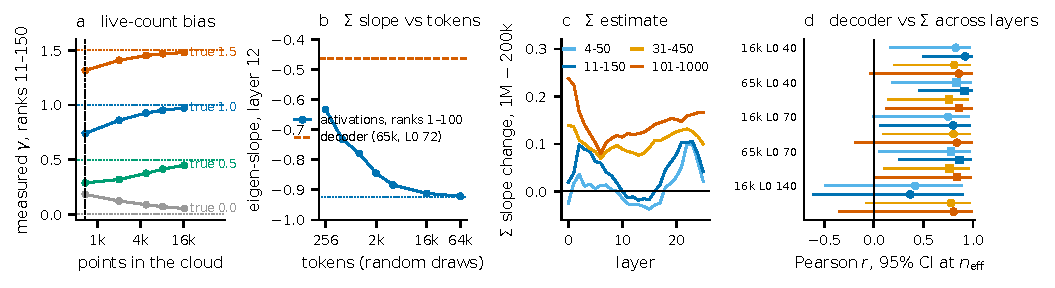
\includegraphics[width=\textwidth]{thesisB_fig3_estimator.pdf}
\caption{\textbf{Properties of the estimator.} (a) Measured $\gam$ (ranks 11--150) of Gaussian clouds whose covariance is $\Sigma_{13}^{\gam}$ for a known $\gam$ (dotted), against the number of points, $d$ = 2,304, 6 draws (sd $\le$ 0.011). Dashed: 672 points, the live count of our $k = 1$ SAEs. (b) Layer 12: activation-covariance slope (ranks 1--100) against the number of randomly drawn tokens (3 draws), with the 1M-token value (dotted) and Li et al.'s decoder (dashed). (c) Change in $\Sigma$'s slope from 200k to 1M tokens at each layer, by window. (d) Pearson $r$ between decoder and $\Sigma$ slopes across 26 layers, with 95\% intervals using the effective sample size; colours as in (c), circles 16k, squares 65k.}
\label{fig:estimator}
\end{figure*}

\paragraph{Live-count bias.} A cloud of $n$ points in $d$ = 2,304 dimensions has sampling noise in every eigenvalue, which pulls steep spectra toward flat and lifts flat ones. We simulated unit-normalised Gaussian clouds with covariance $\Sigma_{13}^{\gam}$ for known $\gam$ (Figure~\ref{fig:estimator}a). In ranks 11--150 a true $\gam$ of 1.0 measures 0.741 at 672 points, 0.928 at 4,786 and 0.974 at 16,384. A true 0 (isotropic) measures 0.183, 0.089 and 0.054. The bias is not negligible even at full width: a true 0.5 measures 0.450 at 16,384 points. Inverting this calibration, our $k = 1$ SAE's measured $\gam$ of 1.034 (672 live latents) corresponds to about 1.25, and the corrected $k$ sweep falls by 0.115 per doubling rather than 0.094 (Appendix~\ref{app:live}). The correction assumes a Gaussian cloud with power-law covariance, so it is approximate. For Gemma Scope the bias acts through width, since a wider SAE contributes more rows. Rescoring all 28 layer-12 SAEs on 16,384 random rows each changes the per-doubling L0 coefficient from 0.099 to 0.096 and no single slope by more than 0.037 in ranks 11--150. In ranks 101--1000 the effect is larger (up to 0.060), which is part of the width effect there.

\paragraph{How many tokens $\Sigma$ needs.} Too few documents make the bulk of $\Sigma$'s spectrum too steep, and too few random tokens make its top too flat. At layer 12, two document-disjoint halves of a 1M-token sample agree to within 0.003 in every window, while the first 200k tokens (about 200 documents) are steeper than the full sample by 0.08 (ranks 31--450) and 0.12 (ranks 101--1000). Over all 26 layers the 200k estimate is steeper than the 1M one by 0.10 and 0.14 on average in the bulk windows, and by up to 0.24 at a single layer (Figure~\ref{fig:estimator}c). In the top windows the mean difference is 0.01--0.04 but reaches 0.10 at layers 21--23. Estimated from 200k tokens, the layer correlations of Section~\ref{sec:gamma} drop from 0.75--0.92 to 0.52--0.79. In the other direction, random draws of a few thousand tokens flatten the top of the spectrum (ranks 1--100: $-0.884$ at 4,096 tokens against $-0.921$ at 65,536; Figure~\ref{fig:estimator}b). Any $\gam$ is only as good as its denominator.

\paragraph{Correlations across layers.} Adjacent layers are not independent: both the decoder and $\Sigma$ slope profiles are smooth humps. Using the lag correlations of both series, the effective sample size behind a 26-layer Pearson $r$ is 4.8--8.4 (Figure~\ref{fig:estimator}d). With that correction, the correlations at L0 = 40 and 70 have $p$ = 0.003--0.09 and 95\% intervals whose lower ends run from $-0.18$ to 0.50; phase-randomised surrogates agree (Appendix~\ref{app:r}). A correlation over layers should be quoted with its interval, not to two decimals.

\paragraph{Smaller choices.} Using named instead of measured L0 changes interpolated layer profiles by at most 0.021. Seed-to-seed spread of our TopK slopes is at most 0.014 in ranks 11--150. Table~\ref{tab:ledger} collects these effects next to the large ones.

\begin{table}[t]
\centering
\small
\caption{\textbf{How much each factor moves the slope} (ranks 11--150 unless stated). Large effects at the top, choices that barely matter at the bottom.}
\label{tab:ledger}
\begin{tabular}{@{}p{0.74\columnwidth}@{\hspace{4pt}}r@{}}
\toprule
Factor & Change \\
\midrule
L0 over Gemma Scope's range (9--457), pooled & 0.46 \\
L0, one doubling, layer 12, 7 widths & 0.099 \\
L0, one doubling, single 16k ladders (layer 2 to 15) & 0.021--0.129 \\
$k$, one doubling, our TopK, layer 13 ($k$ 8--128) & 0.092 \\
Layer, across 26 layers at fixed L0 (16k; L0 40, 140) & 0.24, 0.16 \\
Rank window, one SAE (Li et al.'s layer 12) & 0.085 \\
Width, 16k to 1M at fixed L0 (L0 40, 70) & $\le$ 0.051 \\
\quad same, ranks 101--1000 & 0.13--0.14 \\
Rows: 1M-wide decoder cut to 16,384 rows & 0.028--0.038 \\
$\Sigma$ from 200k vs 1M tokens ($\Sigma$ slope; any layer) & $\le$ 0.105 \\
\quad same, ranks 101--1000 & $\le$ 0.24 \\
\midrule
Named vs measured L0 (16k layer profiles) & $\le$ 0.021 \\
Seed (our TopK, 2--3 seeds) & $\le$ 0.014 \\
Near-duplicate latents removed (up to 35\%) & $\le$ 0.010 \\
Massive-activation tokens dropped in training & $\le$ 0.005 \\
Centring the rows & $\le$ 0.0007 \\
Latents aligned with dims 1170, 334 removed & $\le$ 0.0002 \\
\bottomrule
\end{tabular}
\end{table}

\section{What the exponent does not reflect}
\label{sec:not}

\paragraph{Near-duplicate latents.} One might expect the leading eigenvalues to come from groups of near-parallel latents, as produced by feature splitting \citep{chanin2025absorption}. At layer 12, 2--59\% of latents have a neighbour at cosine above 0.5, more at low L0. Greedily merging latents above that threshold removes up to 35\% of a dictionary (131k, L0 12) and changes the slope by at most 0.010 in ranks 11--150 and 0.012 in ranks 4--50 across 22 SAEs. In the bulk windows it changes it by up to 0.029 and 0.051, partly because the cloud has fewer rows. The anisotropy is spread through the cloud, not concentrated in duplicates.

\paragraph{Massive activations.} Gemma-2-2B's residual stream has a few dimensions that take rare, very large values, the phenomenon described by \citet{sun2024massive}; we test two such dimensions, 1170 and 334. Every layer-12 Gemma Scope SAE we checked (10 SAEs, 16k and 65k) has latents aligned with these dimensions (maximum $|\cos|$ 0.81--0.97, against at most 0.12 for a control dimension). Removing all latents with $|\cos| > 0.2$ to either one (at most 18) changes the slope by at most 0.0002. Retraining our layer-13 TopK SAE without the tokens carrying the top 0.1\% or 1\% of $|x_{1170}|$ changes its slope by at most 0.005 in every window (3 seeds).

\paragraph{Latent firing frequencies.} Over the 22 layer-12 SAEs whose firing we measured on 1M tokens, the rank--frequency exponent of latent firing rates (ranks 10 to the last live latent) runs from $-1.01$ to $-0.59$ and correlates with the decoder slope at $r = -0.47$. In ranks 10--100 of the frequency curve the correlation is 0.18. The frequency distribution is therefore not a proxy for the decoder exponent. Latent frequencies are not feature frequencies, so this does not test allocation models such as \citet{michaud2025manifolds}.

\paragraph{A covariance-matched Gaussian null (secondary evidence).} If the exponent were fixed by $\Sigma$ and the sparsity level, an SAE trained on $N(\mu,\Sigma)$ should reproduce it. Table~\ref{tab:null} compares raw decoder slopes of real and Gaussian-trained TopK SAEs at layers 3, 13 and 23 ($k$ = 40, 3 seeds, sd $\le$ 0.009). The Gaussian SAE does not reproduce the real layer profile: in ranks 11--150 its slope steepens monotonically with depth ($-0.424$, $-0.505$, $-0.507$) while real data peaks at layer 13 ($-0.290$, $-0.481$, $-0.292$). In the bulk windows the Gaussian slopes are 2.1--4.7 times steeper than real ones at every layer. Of 24 (width, window, layer) cells, real and Gaussian agree within 0.03 in three: layer 13 in ranks 11--150 at 16k, and layers 3 and 23 in ranks 4--50 at 65k. In the layer-13 $k$ sweep they agree within 0.03 at $k$ = 40 and 128, but the Gaussian slope is not monotone in $k$ ($-0.424$ at $k$ = 16, $-0.507$ at $k$ = 40). This evidence covers three layers, one $k$ and one model, so we use it only to say that $\Sigma$ and L0 together do not determine the exponent; real activations carry structure that a Gaussian with the same covariance lacks.

\begin{table}[t]
\centering
\small
\caption{\textbf{Real versus covariance-matched Gaussian SAEs}: raw decoder slope, 16k, $k$ = 40, mean of 3 seeds. The 65k runs and $\gam$ values are in Appendix~\ref{app:null}.}
\label{tab:null}
\begin{tabular}{llccc}
\toprule
Ranks & Training data & L3 & L13 & L23 \\
\midrule
4--50 & real & $-0.224$ & $-0.475$ & $-0.340$ \\
 & Gaussian & $-0.255$ & $-0.276$ & $-0.286$ \\
11--150 & real & $-0.290$ & $-0.481$ & $-0.292$ \\
 & Gaussian & $-0.424$ & $-0.505$ & $-0.507$ \\
31--450 & real & $-0.554$ & $-0.446$ & $-0.280$ \\
 & Gaussian & $-1.181$ & $-1.050$ & $-0.972$ \\
101--1000 & real & $-0.676$ & $-0.571$ & $-0.389$ \\
 & Gaussian & $-2.394$ & $-1.921$ & $-1.841$ \\
\bottomrule
\end{tabular}
\end{table}

\section{Discussion}
\label{sec:discussion}

The decoder power-law exponent is a joint property of the layer's activations, the SAE's sparsity and the part of the spectrum one fits. In the window where it has been reported, sparsity is the largest of these; deeper in the spectrum, layer is. A layer comparison made with SAEs of different L0, or in different windows, mixes these effects. Gemma Scope makes the L0 problem easy to fall into, because its released ladders have different L0 values at different layers. Expressing the exponent relative to $\Sigma$ does not remove the dependence on sparsity, and it adds an estimation problem in the denominator.

\paragraph{Reporting checklist.} For anyone who reports this statistic:
\begin{itemize}
\setlength{\itemsep}{0pt}
\item State L0 (measured, not only named) and compare layers or models only at matched L0, interpolating along a ladder if needed.
\item Report the rank window, and at least one top and one bulk window; they can disagree in sign of the layer trend.
\item Report the number of rows in the cloud, and compare clouds at a fixed row count; below a few thousand live rows, apply a calibration such as Figure~\ref{fig:estimator}a.
\item If dividing by $\Sigma$'s slope, estimate $\Sigma$ from at least 1M tokens drawn by document, and check split halves.
\item Quote correlations across layers with an interval at the effective sample size.
\end{itemize}

\paragraph{Limitations.} Everything here is one model, Gemma-2-2B, and one SAE family for the population analysis; we have not tested whether the per-doubling rate transfers to other models or SAE suites. Gemma Scope's L0 is confounded with each SAE's training run, and our controlled $k$ sweep is one layer, one width and two seeds. The decomposition is linear in $\log$ L0 with additive layer effects; the interaction term shows the L0 effect varies by layer, so the single per-doubling number is an average. The live-count correction assumes Gaussian clouds. $\Sigma$ is estimated from Pile text, not Gemma Scope's training mixture, which may bias $\gam$ by an unknown amount; the decoder slopes do not depend on this. The Gaussian-null comparison covers three layers at one $k$. Our search of related work covered the decoder-spectrum and SAE-null literature; we have not found prior work separating L0 from layer for this statistic, but cannot rule it out.

\paragraph{What is open.} Three experiments would sharpen these conclusions: real and Gaussian-trained SAEs at matched $k$ across more layers, to separate the parts of the layer profile that $\Sigma$ and real structure produce; a denser $k$ sweep with more seeds, scored at a fixed live count; and SAEs trained on whitened activations. Each has a place above (Table~\ref{tab:null}, Figure~\ref{fig:main}c, Section~\ref{sec:gamma}).

\section{Conclusion}

Li et al.'s slopes reproduce exactly, and the power law is there. But the number they compared across layers is mainly a number about sparsity in their window, about layer in the bulk, and about the window everywhere. Quoted with its L0, its window and its row count, it is a useful and stable measurement; quoted alone, it describes the SAE as much as the layer.

\section*{Impact Statement}
This paper re-measures a descriptive statistic of sparse autoencoders and documents how to compute it reliably. It introduces no new capability. Its main effect is methodological: interpretability claims that rest on this statistic should become more comparable and less prone to artefacts of SAE choice. We see no direct negative societal consequences.

{\small
\bibliographystyle{plainnat}
\bibliography{thesisB}
}

\clearpage
\onecolumn
\appendix

\section{Methods}
\label{app:methods}

\paragraph{Gemma Scope SAEs.} Release \texttt{gemma-scope-2b-pt-res} (JumpReLU). Decoder matrices only, except where measured L0 or firing frequencies are needed. Spectra use the full decoder (all rows, dead ones included), centred covariance with $n-1$ normalisation, eigenvalues sorted in decreasing order. Fits are ordinary least squares of $\log_{10}\lambda$ on $\log_{10}$ rank. In code, windows are 0-based slices: ranks 11--150 is the slice [10, 150).

\paragraph{Measured L0.} For the 135 16k SAEs: JumpReLU encoder applied to 32,736 Pile tokens (32 sequences of 1,024), firing = pre-activation above threshold. Measured over named L0 lies in 0.85--1.12; its median per layer lies in 0.92--1.11, highest at layers 10--15. For layer 12, 22 SAEs were measured on 1M tokens; the remaining 6 use named L0. Refitting the 16k-only decomposition with measured instead of named L0 changes the per-doubling coefficient by at most 0.004 and the $R^2$ of the L0-plus-layer model by at most 0.011:

\begin{center}
\small
\begin{tabular}{lcccc}
\toprule
16k SAEs, 135 & 4--50 & 11--150 & 31--450 & 101--1000 \\
\midrule
$b$ per doubling, named / measured & 0.085 / 0.089 & 0.077 / 0.080 & 0.065 / 0.067 & 0.062 / 0.064 \\
$R^2$ (L0 + layer), named / measured & 0.88 / 0.89 & 0.87 / 0.88 & 0.96 / 0.96 & 0.93 / 0.93 \\
\bottomrule
\end{tabular}
\end{center}

\paragraph{Interpolation to fixed L0.} For each layer and width, slope is interpolated linearly in $\log$ L0 between the two SAEs whose L0 brackets the target. Layers whose ladder does not bracket the target are omitted (L0 = 20 is bracketed at 11 layers for 16k; L0 = 140 at 24 layers for 65k).

\paragraph{Activation covariance.} Residual stream after each block of Gemma-2-2B, Pile (uncopyrighted subset), context 1,024, beginning-of-sequence position dropped, 1,002,540 tokens for the 26-layer $\Sigma$. The 200k comparison uses the first 200,508 tokens. Split halves at layer 12 are by document (even and odd sequences).

\paragraph{Our TopK SAEs.} TopK activation with the AuxK loss ($k_{\text{aux}}$ = 512, coefficient 1/32, dead window 2M tokens), unit-norm decoder rows with the parallel gradient component removed, Adam with learning rate $2\times10^{-4}\sqrt{16384/\text{width}}$ and linear decay over the last 20\% of steps, batch 4,096, inputs scaled so that $\mathbb{E}\|x\|^2 = d$. For each of layers 3, 13 and 23, 10M Pile tokens were cached, the last 0.5M held out for evaluation; training ran 3 epochs over the remaining 9.5M (28.5M token presentations). The Gaussian null samples $N(\mu,\Sigma)$ with $\mu$ and $\Sigma$ from those 10M tokens. Evaluation fraction of variance unexplained at $k$ = 40, 16k: 0.288 (layer 13, real). $\gam$ for these SAEs uses the 10M-token $\Sigma$.

\paragraph{Effective sample size.} $n_{\text{eff}} = n/(1 + 2\sum_{k=1}^{K} r_x(k)\,r_y(k))$ with lags up to $K = \lfloor n/4 \rfloor$, clipped to [3, $n$]; Fisher-$z$ intervals use $n_{\text{eff}}-3$. Phase-randomised surrogates (10,000) randomise the Fourier phases of the decoder series. These choices were fixed before computing the results.

\section{Reproduction}
\label{app:repro}

\begin{table}[h]
\centering
\small
\caption{Li et al.'s notebook SAEs (65k), ranks 11--150, and the same SAEs in other fit ranges.}
\label{tab:repro}
\begin{tabular}{lcccccccc}
\toprule
Layer (L0) & Li et al. & Ours & Rel.\ diff. & $R^2$ & ranks 2--15 & 4--50 & 31--450 & 101--1500 \\
\midrule
0 (73) & $-0.2383$ & $-0.2383$ & 0.019\% & 0.999 & $-0.250$ & $-0.220$ & $-0.263$ & $-0.375$ \\
12 (72) & $-0.4684$ & $-0.4684$ & 0.008\% & 0.994 & $-0.373$ & $-0.476$ & $-0.418$ & $-0.570$ \\
24 (124) & $-0.2545$ & $-0.2545$ & 0.013\% & 0.999 & $-0.181$ & $-0.251$ & $-0.238$ & $-0.343$ \\
\bottomrule
\end{tabular}
\end{table}

\section{\texorpdfstring{$\gamma$}{gamma} across layers}
\label{app:gamma}

$\gam$ of Gemma Scope 65k SAEs at L0 = 40 (1M-token $\Sigma$), mean over layers 0--3, 12--16 and 23--24: ranks 4--50: 0.42, 0.60, 0.49; ranks 11--150: 0.44, 0.64, 0.48; ranks 31--450: 0.55, 0.65, 0.45; ranks 101--1000: 0.58, 0.72, 0.50. Range of $\gam$ over the 26 layers for each cell: 16k L0 40: 0.38--0.59, 0.45--0.61, 0.44--0.72, 0.54--0.83 in the four windows; 65k L0 40: 0.39--0.62, 0.41--0.65, 0.42--0.71, 0.48--0.78; 16k L0 70: 0.31--0.49, 0.37--0.51, 0.36--0.65, 0.47--0.75; 65k L0 70: 0.30--0.54, 0.33--0.54, 0.37--0.67, 0.43--0.74. The layer-12 $\gam$ law in the other windows: ranks 4--50, $1.137 - 0.105\log_2$ L0 ($R^2$ 0.97); ranks 31--450, $1.075 - 0.079\log_2$ L0 (0.95); ranks 101--1000, $1.021 - 0.053\log_2$ L0 (0.65).

\section{Cross-layer correlations}
\label{app:r}

\begin{table}[h]
\centering
\small
\caption{Pearson $r$ between Gemma Scope decoder slope and 1M-token $\Sigma$ slope over 26 layers, with effective sample size, Fisher-$z$ $p$ and 95\% interval at $n_{\text{eff}}$, and phase-surrogate $p$ (``$<$1e-4'': none of 10,000 surrogates as extreme).}
\label{tab:rcells}
\begin{tabular}{llccccc}
\toprule
Cell & Ranks & $r$ & $n_{\text{eff}}$ & $p$ ($n_{\text{eff}}$) & 95\% CI & $p$ (phase) \\
\midrule
16k, L0 40 & 4--50 & 0.826 & 6.8 & 0.022 & [0.17, 0.97] & $<$1e-4 \\
 & 11--150 & 0.922 & 6.5 & 0.003 & [0.50, 0.99] & $<$1e-4 \\
 & 31--450 & 0.811 & 7.6 & 0.015 & [0.21, 0.97] & 0.021 \\
 & 101--1000 & 0.857 & 5.2 & 0.055 & [$-$0.03, 0.99] & 0.080 \\
16k, L0 70 & 4--50 & 0.750 & 7.0 & 0.051 & [0.00, 0.96] & 0.024 \\
 & 11--150 & 0.802 & 6.6 & 0.037 & [0.07, 0.97] & 0.023 \\
 & 31--450 & 0.804 & 6.8 & 0.031 & [0.10, 0.97] & 0.051 \\
 & 101--1000 & 0.837 & 5.0 & 0.089 & [$-$0.18, 0.99] & 0.127 \\
16k, L0 140 & 4--50 & 0.418 & 7.0 & 0.373 & [$-$0.49, 0.89] & 0.447 \\
 & 11--150 & 0.369 & 6.2 & 0.491 & [$-$0.61, 0.90] & 0.602 \\
 & 31--450 & 0.778 & 6.1 & 0.067 & [$-$0.07, 0.97] & 0.143 \\
 & 101--1000 & 0.805 & 4.8 & 0.141 & [$-$0.35, 0.99] & 0.176 \\
65k, L0 40 & 4--50 & 0.835 & 6.8 & 0.019 & [0.19, 0.98] & $<$1e-4 \\
 & 11--150 & 0.916 & 6.4 & 0.004 & [0.46, 0.99] & $<$1e-4 \\
 & 31--450 & 0.760 & 8.4 & 0.020 & [0.15, 0.95] & 0.037 \\
 & 101--1000 & 0.862 & 5.8 & 0.029 & [0.13, 0.99] & 0.068 \\
65k, L0 70 & 4--50 & 0.780 & 7.0 & 0.037 & [0.06, 0.97] & 0.0004 \\
 & 11--150 & 0.864 & 6.5 & 0.014 & [0.26, 0.98] & $<$1e-4 \\
 & 31--450 & 0.764 & 7.8 & 0.028 & [0.11, 0.96] & 0.058 \\
 & 101--1000 & 0.838 & 5.7 & 0.047 & [0.02, 0.98] & 0.103 \\
\bottomrule
\end{tabular}
\end{table}

\section{Live-count calibration and the corrected \texorpdfstring{$k$}{k} sweep}
\label{app:live}

\begin{table}[h]
\centering
\small
\caption{Left: measured $\gam$ (ranks 11--150) of unit-normalised Gaussian clouds with covariance $\Sigma_{13}^{\gam}$, by number of points (6 draws, sd $\le$ 0.011). Right: our layer-13 TopK SAEs (2 seeds): live latents, measured $\gam$, and $\gam$ corrected by inverting the calibration at each SAE's live count.}
\label{tab:live}
\begin{tabular}{lccccc}
\toprule
True $\gam$ & 672 & 2,000 & 4,786 & 8,192 & 16,384 \\
\midrule
0 & 0.183 & 0.123 & 0.089 & 0.071 & 0.054 \\
0.25 & 0.200 & 0.151 & 0.143 & 0.153 & 0.176 \\
0.5 & 0.289 & 0.319 & 0.376 & 0.414 & 0.450 \\
0.75 & 0.483 & 0.580 & 0.657 & 0.688 & 0.715 \\
1.0 & 0.741 & 0.861 & 0.928 & 0.953 & 0.974 \\
1.25 & 1.027 & 1.137 & 1.192 & 1.213 & 1.228 \\
1.5 & 1.317 & 1.410 & 1.454 & 1.470 & 1.481 \\
\bottomrule
\end{tabular}
\quad
\begin{tabular}{lcccc}
\toprule
$k$ & live & slope & $\gam$ & corrected \\
\midrule
1 & 672 & $-0.979$ & 1.034 & 1.25 \\
2 & 1,890 & $-0.845$ & 0.893 & 1.04 \\
4 & 3,732 & $-0.780$ & 0.824 & 0.92 \\
8 & 6,469 & $-0.694$ & 0.732 & 0.80 \\
16 & 14,472 & $-0.630$ & 0.665 & 0.71 \\
40 & 16,262 & $-0.482$ & 0.509 & 0.56 \\
128 & 16,384 & $-0.335$ & 0.354 & 0.41 \\
\bottomrule
\end{tabular}
\end{table}

Fits over $k$ = 1--128: measured $\gam = 1.015 - 0.094\log_2 k$ ($R^2$ 0.994); corrected $1.181 - 0.115\log_2 k$ ($R^2$ 0.98). The calibration grid has a step of 0.2 in true $\gam$ with 2 draws and linear interpolation. In ranks 101--1000 the slope is undefined when fewer than 1,000 latents are alive ($k = 1$).

\section{Covariance-matched null: full results}
\label{app:null}

\begin{table}[h]
\centering
\small
\caption{Raw decoder slopes, $k$ = 40, mean of 3 seeds; in parentheses $\gam$ against the 10M-token training $\Sigma$. Training $\Sigma$ slopes (ranks 4--50 / 11--150 / 31--450 / 101--1000): layer 3 $-0.714$ / $-0.676$ / $-0.846$ / $-0.961$; layer 13 $-0.982$ / $-0.947$ / $-0.750$ / $-0.705$; layer 23 $-0.807$ / $-0.749$ / $-0.697$ / $-0.679$.}
\label{tab:nullfull}
\begin{tabular}{lllccc}
\toprule
Width & Ranks & Data & L3 & L13 & L23 \\
\midrule
16k & 4--50 & real & $-0.224$ (0.313) & $-0.475$ (0.484) & $-0.340$ (0.421) \\
 & & Gaussian & $-0.255$ (0.357) & $-0.276$ (0.281) & $-0.286$ (0.355) \\
 & 11--150 & real & $-0.290$ (0.430) & $-0.481$ (0.508) & $-0.292$ (0.389) \\
 & & Gaussian & $-0.424$ (0.627) & $-0.505$ (0.533) & $-0.507$ (0.677) \\
 & 31--450 & real & $-0.554$ (0.655) & $-0.446$ (0.595) & $-0.280$ (0.401) \\
 & & Gaussian & $-1.181$ (1.395) & $-1.050$ (1.401) & $-0.972$ (1.394) \\
 & 101--1000 & real & $-0.676$ (0.703) & $-0.571$ (0.810) & $-0.389$ (0.572) \\
 & & Gaussian & $-2.394$ (2.490) & $-1.921$ (2.726) & $-1.841$ (2.710) \\
65k & 4--50 & real & $-0.218$ (0.305) & $-0.286$ (0.291) & $-0.302$ (0.375) \\
 & & Gaussian & $-0.218$ (0.305) & $-0.228$ (0.232) & $-0.280$ (0.347) \\
 & 11--150 & real & $-0.246$ (0.364) & $-0.366$ (0.387) & $-0.236$ (0.315) \\
 & & Gaussian & $-0.380$ (0.562) & $-0.460$ (0.485) & $-0.497$ (0.663) \\
 & 31--450 & real & $-0.420$ (0.497) & $-0.367$ (0.489) & $-0.204$ (0.292) \\
 & & Gaussian & $-0.915$ (1.082) & $-0.861$ (1.149) & $-0.875$ (1.254) \\
 & 101--1000 & real & $-0.515$ (0.536) & $-0.413$ (0.586) & $-0.273$ (0.402) \\
 & & Gaussian & $-1.481$ (1.540) & $-1.176$ (1.669) & $-1.167$ (1.717) \\
\bottomrule
\end{tabular}
\end{table}

Layer-13 $k$ sweep, ranks 11--150, raw slope of the Gaussian-trained SAE (2 seeds; live latents in parentheses): $k$ = 1: $-1.182$ (447); 2: $-1.224$ (828); 4: $-1.166$ (1,563); 8: $-0.782$ (14,419); 16: $-0.424$ (14,562); 40: $-0.507$ (16,384); 128: $-0.361$ (16,383). Real: see Table~\ref{tab:live}. At layer 13 our real 65k slope in ranks 11--150 differs from the 16k one by 0.115, more than Gemma Scope's widths differ at matched L0 ($\le$ 0.051), which suggests our 65k SAEs are undertrained; we draw no width conclusions from them.

\begin{figure}[h]
\centering
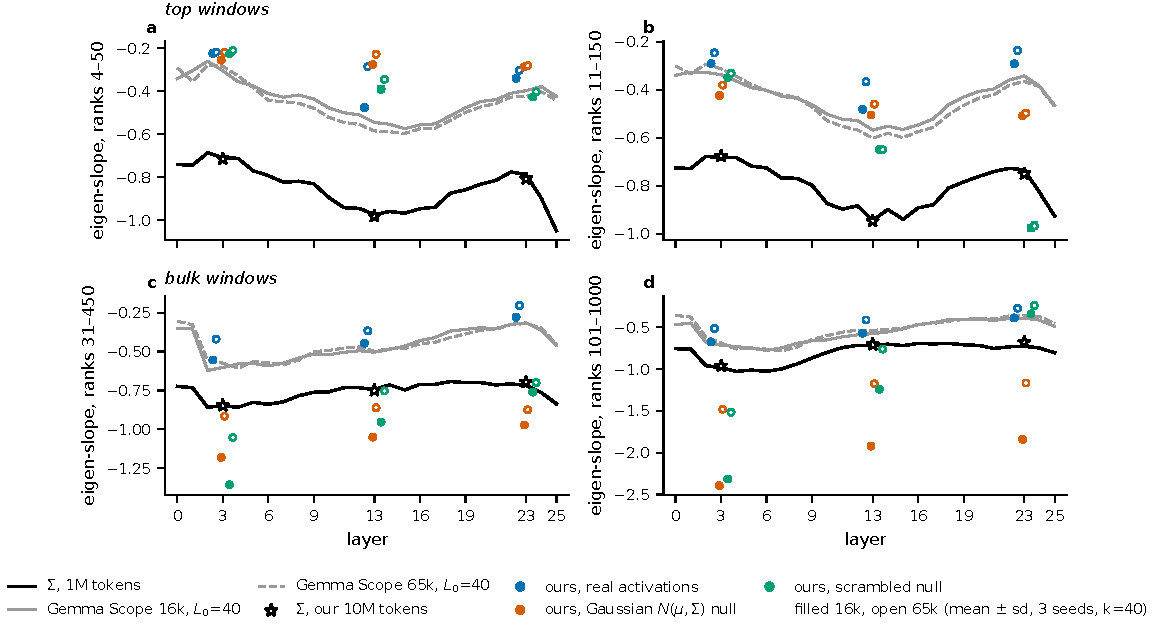
\includegraphics[width=0.9\textwidth]{fig2_layer_profile.pdf}
\caption{Slope against layer in four windows: 1M-token $\Sigma$ (black), Gemma Scope 16k and 65k decoders interpolated to L0 = 40 (grey), the 10M-token training $\Sigma$ of our SAEs (stars), and our TopK $k$ = 40 SAEs trained on real activations, on $N(\mu,\Sigma)$ and on per-coordinate scrambled activations (filled 16k, open 65k; mean $\pm$ sd over 3 seeds, bars smaller than markers). In the bulk windows both nulls are steeper than $\Sigma$ itself while real SAEs are flatter.}
\label{fig:nullprofile}
\end{figure}

The scrambled null (each coordinate permuted independently across tokens) keeps the marginals and destroys correlations. Its slope at layer 23 in ranks 11--150 is $-0.976$, steeper than at layers 3 and 13, and diag($\Sigma$) at layer 23 ($-0.905$) is not flat, so we cannot explain this value; we report it and do not use the scrambled null elsewhere.

\section{Matrix-level test of the \texorpdfstring{$\Sigma^{\gamma}$}{Sigma-gamma} reading}
\label{app:matrix}

For the five layer-12 16k SAEs we rotated the decoder covariance into the eigenbasis of the 1M-token $\Sigma$ and measured (i) the share of its squared entries on the diagonal, (ii) the overlap of the top-10 eigen-subspaces of decoder and $\Sigma$, and (iii) the $R^2$ of $\log$ diagonal against $\log \lambda_\Sigma$. Benchmarks: an exact $\Sigma^{\gam}$ cloud of 16,384 unit rows, and the decoder's own eigenvalues placed in a random basis.

\begin{center}
\small
\begin{tabular}{lccccc}
\toprule
L0 (measured) & 23 & 43 & 84 & 181 & 444 \\
\midrule
Diagonal share: real / exact / random & 0.73 / 0.98 / 0.24 & 0.73 / 0.96 / 0.36 & 0.75 / 0.93 / 0.48 & 0.77 / 0.91 / 0.59 & 0.73 / 0.90 / 0.62 \\
Top-10 overlap: real / exact & 0.62 / 0.99 & 0.52 / 0.98 & 0.41 / 0.98 & 0.19 / 0.95 & 0.12 / 0.92 \\
$R^2$, ranks 11--150 / 101--1000 (real) & 0.975 / 0.989 & 0.967 / 0.983 & 0.944 / 0.976 & 0.730 / 0.972 & 0.013 / 0.955 \\
$R^2$, random basis (max) & 0.002 & 0.002 & 0.003 & 0.012 & 0.006 \\
\bottomrule
\end{tabular}
\end{center}

The $\Sigma^{\gam}$ description holds approximately in ranks 101--1000 at every L0, and in ranks 11--150 only up to L0 of about 84; it is never as diagonal as an exact $\Sigma^{\gam}$ cloud.

\section{Does the \texorpdfstring{$k$}{k} dependence need Gemma Scope's specific directions?}
\label{app:control}

We resynthesised layer-12 activations from the codes of Gemma Scope's 65k L0-72 SAE, with its decoder rows permuted (D), or with rows replaced by Gaussian directions matching their mean and covariance (G), and trained TopK SAEs at $k$ = 8, 16, 32, 64, 128 (one seed, one draw of directions), scored on 8,192 random live latents (4 draws). Raw slopes in ranks 11--150: D $-0.653$, $-0.497$, $-0.380$, $-0.331$, $-0.255$; G $-0.627$, $-0.420$, $-0.336$, $-0.349$, $-0.302$. G's per-doubling flattening is 0.75 of D's over $k$ = 8--128 but 0.44 over $k$ = 16--128, because G is nearly flat after $k$ = 16. With one seed and one draw, this does not settle whether the specific directions matter beyond their covariance.

\section{Frequencies and near-duplicates: details}
\label{app:freq}

Firing frequencies: 22 layer-12 SAEs (widths 16k--131k), 1M tokens, JumpReLU firing rule. Full-range rank--frequency exponent $-1.01$ to $-0.59$; in ranks 10--100, $-1.17$ to $-0.39$. Regressed on $\log_2$ L0, the full-range exponent changes by $-0.043$ per doubling ($R^2$ 0.29). Near-duplicates: random-order greedy merge at cosine 0.5 over the same 22 SAEs; maximum change in slope 0.012, 0.010, 0.029 and 0.051 in the four windows; the largest removal is 34.5\% of the 131k L0-12 SAE.

\end{document}
